\section{概述}
\label{sec:introduction}

\begin{frame}
  \begin{center}
    \Huge{\textcolor{red}{概述}}
  \end{center}
\end{frame}

\subsection{软件设计}

\begin{frame}
  \begin{center}
    \huge{\textcolor{red}{什么是软件设计?}}
  \end{center}
\end{frame}

\begin{frame}{人类认知}
  \begin{figure}
    \centering
    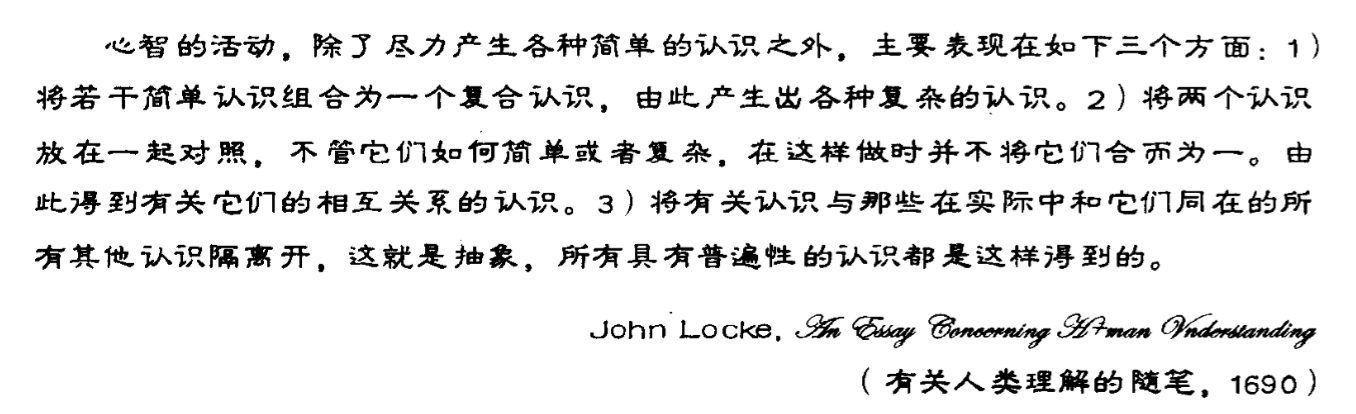
\includegraphics[width=0.8\textwidth]{cognition.png}
  \end{figure}
\end{frame}

\begin{frame}{软件设计:分离与组合的过程}
  \begin{itemize}
    \item \alert{原子}
    \item \alert{组合}
  \end{itemize}
\end{frame}

\begin{frame}
  \begin{center}
    \huge{\textcolor{red}{什么是好的软件设计?}}
  \end{center}
\end{frame}

\begin{frame}{简单设计}
  \begin{block}{以下4个原则的重要程度依次降低}
    \begin{enumerate}
    \item \alert{完成功能}:通过测试
    \item \alert{易于重用}:没有重复
    \item \alert{易于理解}:意图明确
    \item \alert{没有冗余}:恰如其分
    \end{enumerate}
  \end{block}
\end{frame}

\begin{frame}{没有冗余}
  \begin{enumerate}
    \item \alert{YAGNI}: You Ain't Gonna Need It
    \item \alert{KISS}: Keep it Simple, Stupid
  \end{enumerate}
\end{frame}

\begin{frame}{易于理解}
  \begin{enumerate}
    \item \alert{Clean Code}:整洁代码
    \item \alert{Idioms}:习惯用法
    \item \alert{Patterns}:实现模式
  \end{enumerate}
\end{frame}

\begin{frame}{易于重用}
    \begin{enumerate}
    \item \alert{局部化}
    \item \alert{高内聚低耦合}
    \item \alert{正交设计}
    \item \alert{组合设计}
    \end{enumerate}
\end{frame}

\subsection{正交设计}

\begin{frame}{正交设计}
    \begin{enumerate}
    \item \alert{消除重复}
    \item \alert{分离变化}
    \item \alert{缩小依赖范围}
    \item \alert{向着稳定的方向依赖}
    \end{enumerate}
\end{frame}

\begin{frame}{正交设计}
  \begin{block}{应对变化} 
    \begin{enumerate}
    \item \alert{一个变化导致多处散弹修改}:消除重复
    \item \alert{多个变化导致一处频繁修改}:分离变化
    \end{enumerate}
  \end{block}

  \begin{block}{变化发生时,消除不必要的修改} 
    \begin{enumerate}
    \item \alert{不依赖不必要的依赖}:缩小依赖范围
    \item \alert{不依赖不稳定的依赖}:向着稳定的方向依赖
    \end{enumerate}
  \end{block}
\end{frame}

\subsection{组合设计}

\begin{frame}{两种模型}
    \begin{enumerate}
    \item \alert{贫血模型}
        \begin{itemize}
        \item 数据和行为的完全分离
        \item 面向过程
        \end{itemize}
    \item \alert{充血模型}
        \begin{itemize}
        \item 高频变化的行为和低频变化数据的耦合
        \item 上帝类
        \end{itemize}
    \end{enumerate}
\end{frame}

\begin{frame}{理解面向对象}
  \begin{block}{类与对象}
    \begin{enumerate}
      \item \alert{类是一种模块化的设计技术}
      \item \alert{对象是对领域的直接映射}
    \end{enumerate}
  \end{block}
\end{frame}

\begin{frame}{小类大对象}
  \begin{figure}
    \centering
    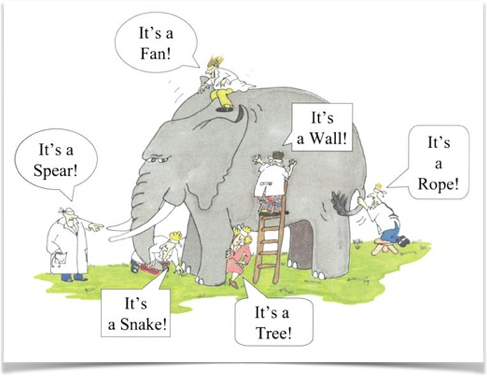
\includegraphics[width=0.7\textwidth]{multi-roles-object.png}
  \end{figure}
\end{frame}

\begin{frame}{多角色对象}
  \begin{figure}
    \centering
    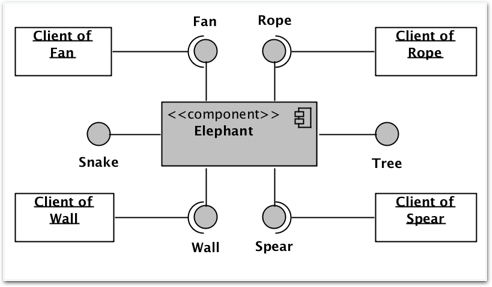
\includegraphics[width=0.7\textwidth]{elephant.png}
  \end{figure}
\end{frame}

\begin{frame}{DCI架构}
  \begin{figure}
    \centering
    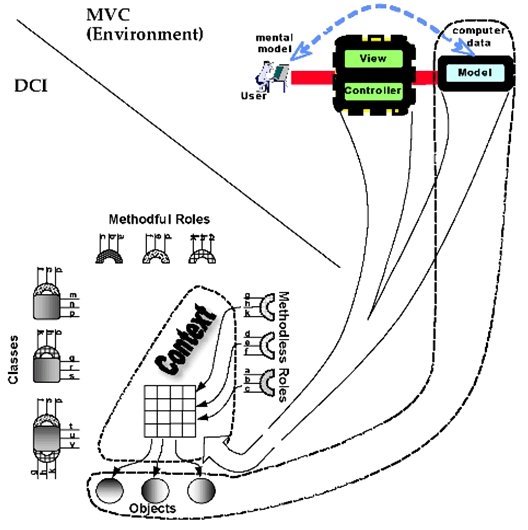
\includegraphics[width=0.55\textwidth]{dci.png}
  \end{figure}
\end{frame}

\begin{frame}{DCI解读}
    \begin{enumerate}
    \item \alert{Data}: What system is?
          \begin{itemize}
          \item Domain Concepts
          \item Relations 
          \item Constraints
          \end{itemize}
    \item \alert{Interaction}: what the system does 
          \begin{itemize}
          \item Algorithm
          \item Business Logic 
          \end{itemize}
    \item \alert{Context}: Comprises \alert{use case} and \alert{algorithms} in which \alert{data object} are used through specific \alert{role}
    \end{enumerate}
\end{frame}
